\documentclass[11pt]{article}

\pdfpagewidth 8.5in
\pdfpageheight 11in

\setlength\topmargin{0in}
\setlength\headheight{0in}
\setlength\headsep{0.4in}
\setlength\textheight{8in}
\setlength\textwidth{6in}
\setlength\oddsidemargin{0in}
\setlength\evensidemargin{0in}
\setlength\parindent{0.25in}
\setlength\parskip{0.1in} 
 
\usepackage{amssymb}
\usepackage{amsfonts}
\usepackage{amsmath}
\usepackage{mathtools}
\usepackage{amsthm}

\usepackage{fancyhdr}

\usepackage{enumerate}

      \theoremstyle{plain}
      \newtheorem{theorem}{Theorem}
      \newtheorem{lemma}[theorem]{Lemma}
      \newtheorem{corollary}[theorem]{Corollary}
      \newtheorem{proposition}[theorem]{Proposition}
      \newtheorem{conjecture}[theorem]{Conjecture}
      \newtheorem{question}[theorem]{Question}
      
      \theoremstyle{definition}
      \newtheorem{definition}[theorem]{Definition}
      \newtheorem{example}[theorem]{Example}
      \newtheorem{game}[theorem]{Game}
      
      \theoremstyle{remark}
      \newtheorem{remark}[theorem]{Remark}



\pagestyle{fancy}
\renewcommand{\headrulewidth}{0.5pt}
\renewcommand{\footrulewidth}{0pt}
\lfoot{\small \jobname.tex -- Updated on \today}
\chead{\small http://github.com/StevenClontz/Research}
\rfoot{\thepage}
\cfoot{}


% Strategy uparrow shortcuts
\newcommand{\win}{\uparrow}
\newcommand{\prewin}{\uparrow_{\text{pre}}}
\newcommand{\markwin}{\uparrow_{\text{mark}}}
\newcommand{\tactwin}{\uparrow_{\text{tact}}}
\newcommand{\ktactwin}[1]{\uparrow_{#1\text{-tact}}}
\newcommand{\kmarkwin}[1]{\uparrow_{#1\text{-mark}}}
\newcommand{\codewin}{\uparrow_{\text{code}}}
\newcommand{\limitwin}{\uparrow_{\text{limit}}}

\newcommand{\oneptcomp}[1]{#1^*}
\newcommand{\oneptlind}[1]{#1^\dagger}

\newcommand{\congame}[2]{Con_{O,P}(#1,#2)}
\newcommand{\clusgame}[2]{Clus_{O,P}(#1,#2)}

\newcommand{\lfkpgame}[1]{LF_{K,P}(#1)}
\newcommand{\lfklgame}[1]{LF_{K,L}(#1)}

\newcommand{\pfgame}[1]{PF_{F,C}(#1)}

\newcommand{\mengame}[1]{Cov_{C,F}(#1)}
\newcommand{\rothgame}[1]{Cov_{C,S}(#1)}
\newcommand{\altrothgame}[1]{Cov_{P,O}(#1)}

\newcommand{\fillgame}[1]{Fill^{\subseteq}_{M,N}(#1)}
\newcommand{\sfillgame}[1]{Fill^{\subsetneq}_{M,N}(#1)}

\newcommand{\kfillgame}[1]{Fill^{\subseteq}_{C,F}(#1)}
\newcommand{\ksfillgame}[1]{Fill^{\subsetneq}_{C,F}(#1)}

\newcommand{\sigmaprodr}[1]{\Sigma\mathbb{R}^{#1}}
\newcommand{\sigmaprodtwo}[1]{\Sigma2^{#1}}

\newcommand{\concat}{^\frown}
\newcommand{\rest}{\restriction}

\newcommand{\cl}[1]{\overline{#1}}

\newcommand{\pow}[1]{\mc{P}(#1)}

\newcommand{\<}{\langle}
\renewcommand{\>}{\rangle}

\newcommand{\mc}[1]{\mathcal{#1}}

\newcommand{\Lim}{\mathrm{Lim}}
\newcommand{\Suc}{\mathrm{Suc}}

\newcommand{\ds}{\displaystyle}

\newcommand{\rank}{\textrm{rank}}

\newcommand{\scish}{$\sigma$-compactish }

\begin{document}

  \begin{question}
    Week 3 (1b) 

    Show that there is no no-trivial chain $\gamma\in C_2(\mc{S}(E),\mathbb{Z})$ whose boundary is in $A$.
  \end{question}

  \centerline{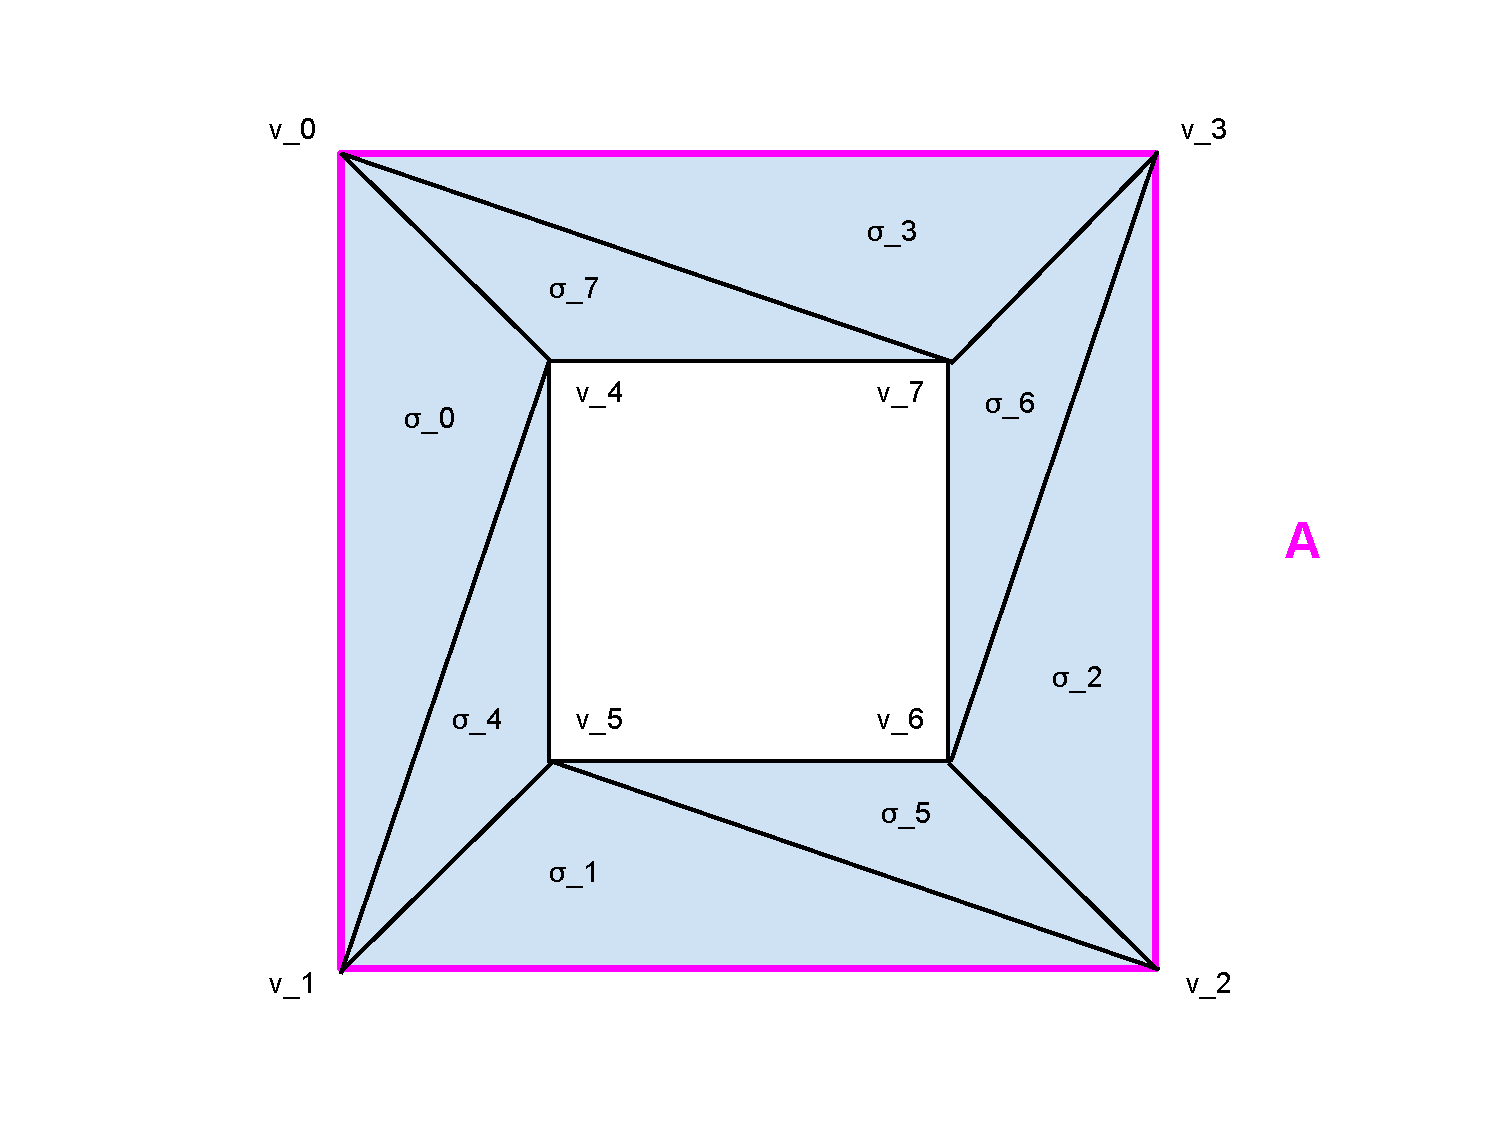
\includegraphics[width=0.7\linewidth]{alg-top-2013-09-18.pdf}}

  \begin{proof}
    Assume $\gamma$ has boundary completely in $A$. Then $\partial(\gamma)=\sum_{i<4} k_i[v_i,v_{i+1(\text{mod}4)}]$.

    We claim $\gamma(\sigma_i) = 0$ for $4\leq i<8$. This can be verified by observing that giving the faces $\sigma_4,\dots,\sigma_7$ nonzero value in $\gamma$ results in non-zero boundary values for the edges on the inner square.

    Next, we observe that since the values for the $45^\circ$ degree diagonals $[v_i,v_{i+4}]$ ($i<4$) in the boundary of $\gamma$ are each $0$, that the two faces at each edge, $\sigma_0$:$\sigma_7$, $\sigma_1$:$\sigma_3$, etc., must be inversely included in $\gamma$. Thus $\gamma(\sigma_0)=-\gamma(\sigma_7)=0$, $\gamma(\sigma_1)=-\gamma(\sigma_4)=0$, etc.

    Therefore $\gamma(\sigma_i)=0$ for $0\leq i<8$.
  \end{proof}

\end{document}


